\documentclass[wide,a4paper,titlepage,12pt] {article}
\usepackage{polski}
\usepackage[UTF8]{inputenc}
\usepackage{listings}
\usepackage{slashbox}
\usepackage[table]{xcolor}
\usepackage{graphicx,pdflscape}
\usepackage{placeins}

\title{Szeregowanie zadań na dowolnej ilości równoległych procesorów}
\author{Jacek Wieczorek (181043)\\Tymon Tobolski (181037) }

% Title page layout (fold)
\makeatletter
\renewcommand{\maketitle}{
  \begin{titlepage}
    \begin{center}
      \vspace*{3cm}
      \LARGE \@title \par
      \vspace{2cm}
      \textit{\small Autorzy:}\par
      \normalsize \@author\par \normalsize
      \vspace{3cm}
      Prowadzący : mgr inż. Karolina Mokrzysz\\
      Poniedziałek TP 11.00 - 13.00\\
      \vspace{3cm}
      Wydział Elektroniki\\ III rok \par
      \vspace{3cm}
      \small \@date
    \end{center}
  \end{titlepage}
}
\makeatother

\begin{document}
  \maketitle
  \section{Opis problemu}
\paragraph{}
 Celem laboratorium jest zaimplementowanie algorytmu szeregowania $n$ zadań na $m$ równolegle działających procesorach $P_{m} || C_{max}$.

  \section{Symbole i oznaczenia}
\paragraph{}
  \begin{itemize}
    \item $m$ - liczba porcesorów
    \item $n$ - liczba zadań
    \item $C_{max}$ - przybliżony, maksymalny czas całkowity
    \item $C$ - czas optymalny
    \item $v$ - wektor współrzędnych $m$-wymiarowych
    \item $v_i$ - współrzędna w $i$-tym wymiarze
    \item $v_{min}$ - minimalna, największa współrzędna 
    \item $t(z)$ - czas wykonania zadnaia $z$
    \item $p(i)$ - lista zadań $i$-tego procesora
    
  \end{itemize}

  \section{Opis algorytmu}
\paragraph{}
  Pierwszy krok algorytmu opiera się na szybkiej, naiwnej metodzie LPT potrzebnej do wyznaczenia przybliżonego, maksymalnego czasu całkowitego (zawsze wiekszego lub równego od optymalnego). Aby rozważyć szeregowanie zadań na $m$ procesorach wymagana jest $m$-wymiarowa struktura danych. Ze wzgledu na poziom skomplikowania implementacji takiej struktury, została ona uproszczona do postaci tablicy jednowymairowej o rozmiarze $(C_{max})^{m}$. W celu zamodelowania wielowymiarowości, współrzędne $m$-wymiarowe są przeliczane na indeks tablicy $j$ i odwrotnie.
  \newline\newline\indent Wzór : 
  \begin{eqnarray*}
    j = \sum_{i=1}^{m} v_i * m^{m-i}
  \end{eqnarray*}
    \newline\newline\indent Przykład : 
  \begin{eqnarray*}
    m &=& 4 \\ v &=& (1,2,3,4) \\
    j &=& 1 * 4^3 + 2 * 4^2 + 3 * 4 + 4 * 1 = 112 
  \end{eqnarray*}

  Kolejnym krokiem jest ustawienie wartości $-1$ we wszystkich komórkach tabeli, oraz wartości $0$ w pierwszej komórce ($v$ = (0,0,...,0)). Dla każdego zadania $z \in \{1,...,n\}$ wyszukujemy kmórkę, której wartość jest równa numerowi poprzedniego zadania (dla $zadania 1$ poszukujemy wartości $0$). Następnie odnaleziony indeks tabeli jest zamienieniany na wektor współrzędnych $v$. W kolejnym kroku, dla każdego $k \in \{1,...,m\}$ obliczany jest nowy wektor współrzędnych $v'$ na podstawie wzoru :
  \begin{eqnarray*}
    v' &=& v\\
    v'_k &=& v'_k + t(z) 
  \end{eqnarray*}
   Jeżeli $v'_k$ jest mniejsze od $C_{max}$ obliczany jest nowy indeks $j'$ na podstawie wektora $v'$ i w komórce tabeli o indeksie $j'$ zapisywany jest numer zadania $z$.
  \newline\newline
  Po rozdzieleniu wszystkich zadań wyszukiwane są te indeksy tabeli, które zawierają wartość $n$. Następnie wszystkie wyszukane indeksy zostają przekonwertowane na wektory współrzędnych. Spośród tych wektorów, wybierany jest ten, który posiada minimalną wartość największej współrzędnej. Ostatnim krokiem algorytmu jest odtworzenie ścieżki przydzielania zadań na poszczególne procesory. Począwszy od znalezionego zadania, aż do $0$, algorytm działa według podanego schematu :
   \begin{eqnarray*}
      &&\forall \ i \in \{1,...,m\} \\
      &&\indent v'' = v_{min} \\
      &&\indent v''_{i} = v''_{i} - z \\
      &&\indent if \ tab[v'' \Rightarrow index] == z-1\\
      &&\indent\indent v_{min} = v'' \\
      &&\indent\indent z = z-1 \\
      &&\indent\indent p(i).add(z) \\
      &&\indent break
    \end{eqnarray*}
     Podany algorytm powtarzaj póki $z>0$\newline\newline
     W momencie zakończenia algorytmu, każdy procesor ma przydzielony optymalny czas wykonywania zadań.
    \section{Analiza wyników}
    \subsection{Stały zestaw zadań i zmienna ilość procesorów}
    \subsubsection{$m \in \{2,...,7\}$, $n=5$, $range \in \{1,...,20\}$}
     \begin{figure}[htbp]
      \begin{center}
       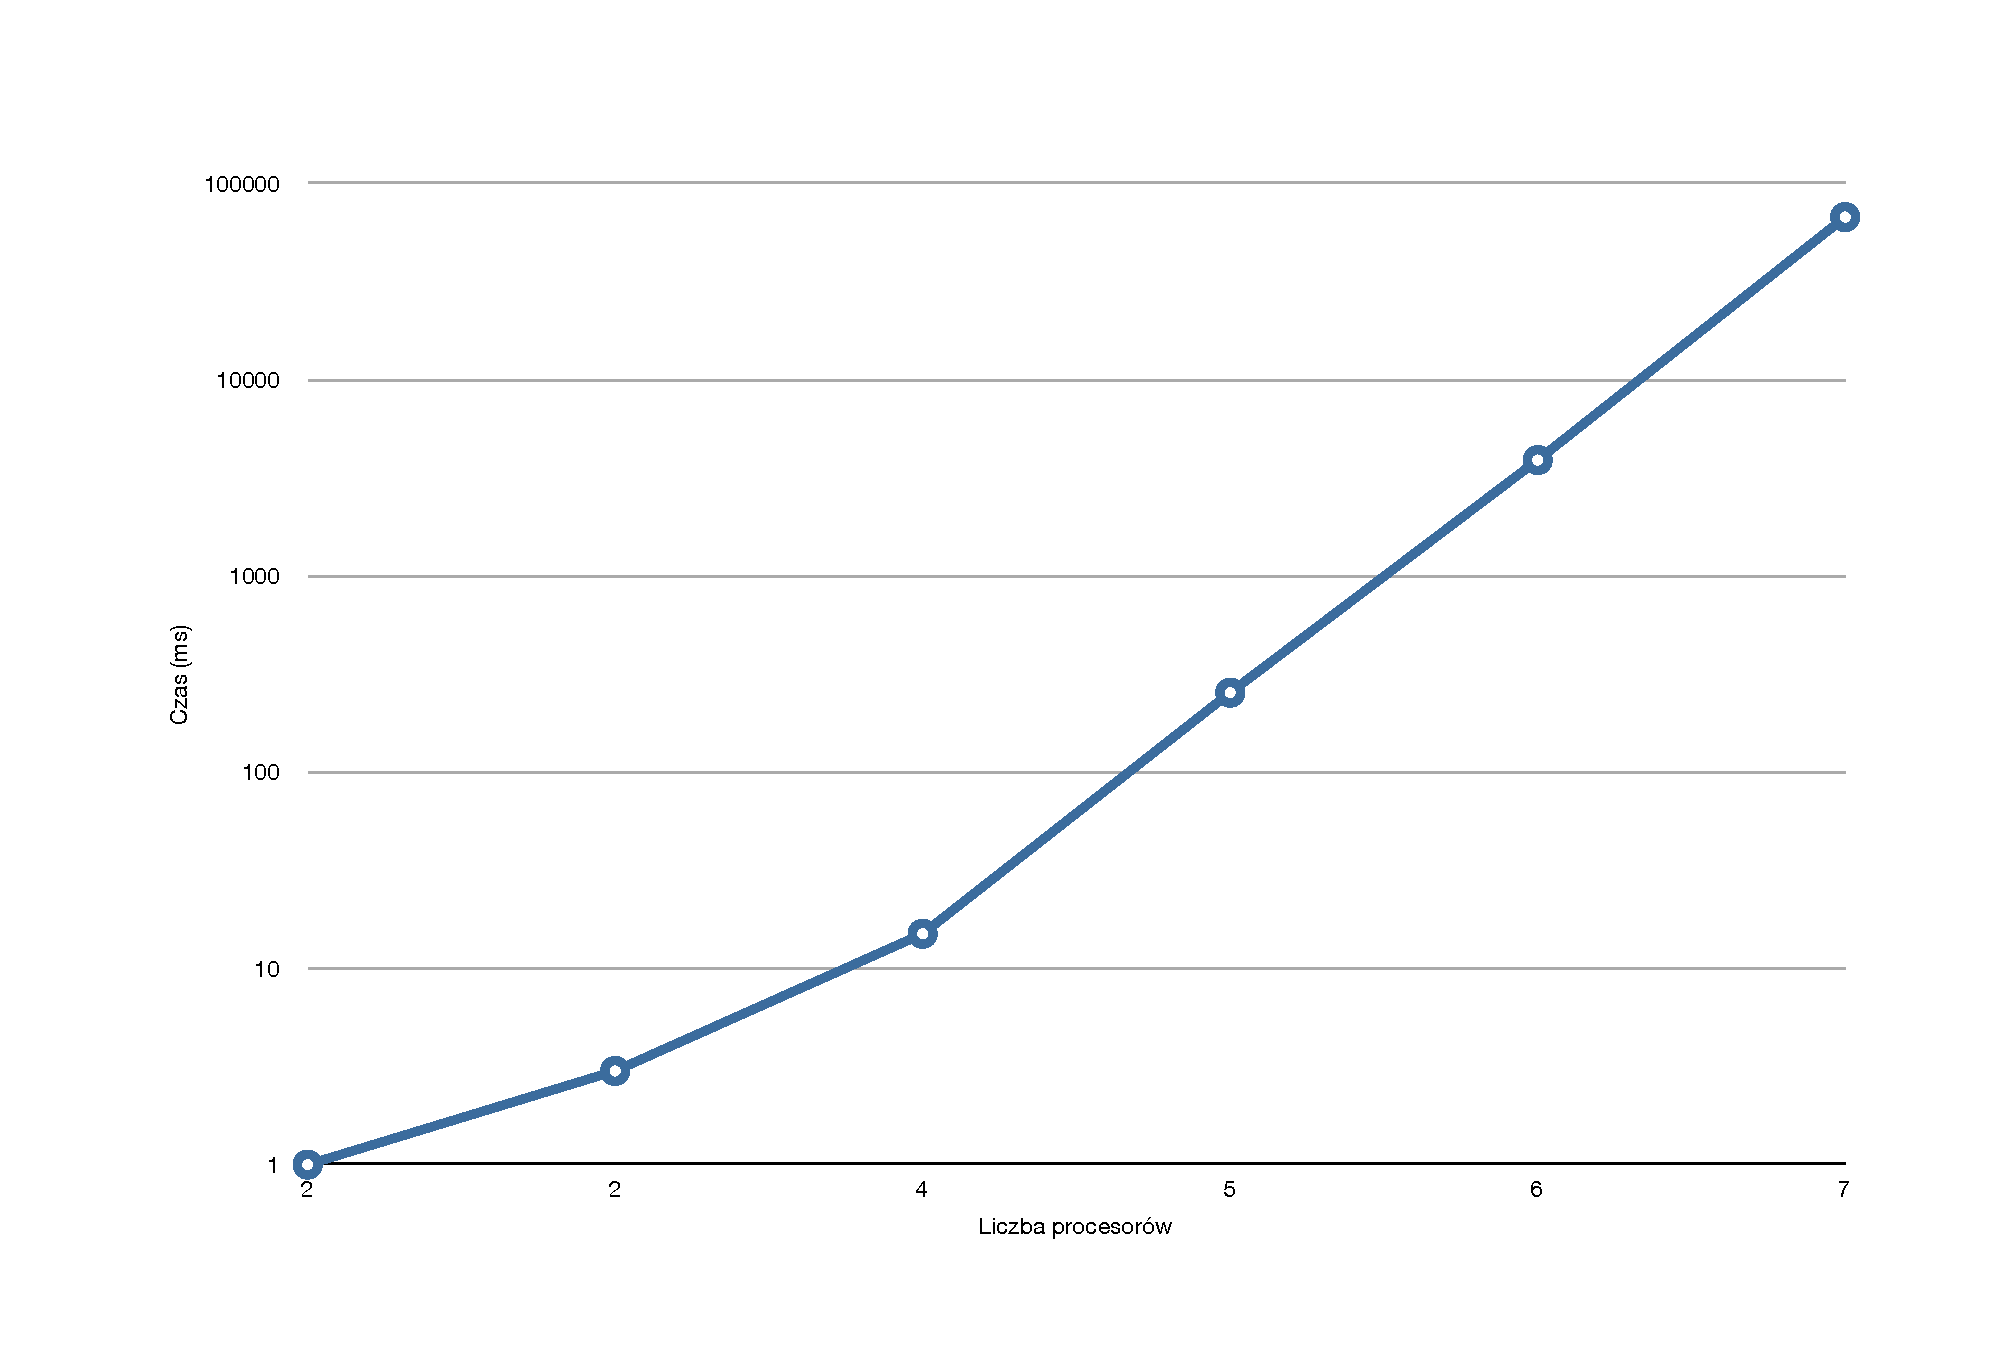
\includegraphics[width=\textwidth]{Fig1.pdf}
        \caption{}
        \label{fig1}
      \end{center}
    \end{figure}
    \begin{center}
    \begin{tabular}{ |c|c| } \hline
      p & T \\ \hline
      2 & 1 \\ 
      3 & 3 \\
      4 & 15 \\
      5 & 254 \\
      6 & 3889 \\
      7 & 67299 \\ \hline
    \end{tabular}
    \end{center}
        \newpage
    \subsubsection{$m \in \{2,...,7\}$, $n=10$, $range \in \{1,...,20\}$}
    \begin{figure}[htbp]
      \begin{center}
       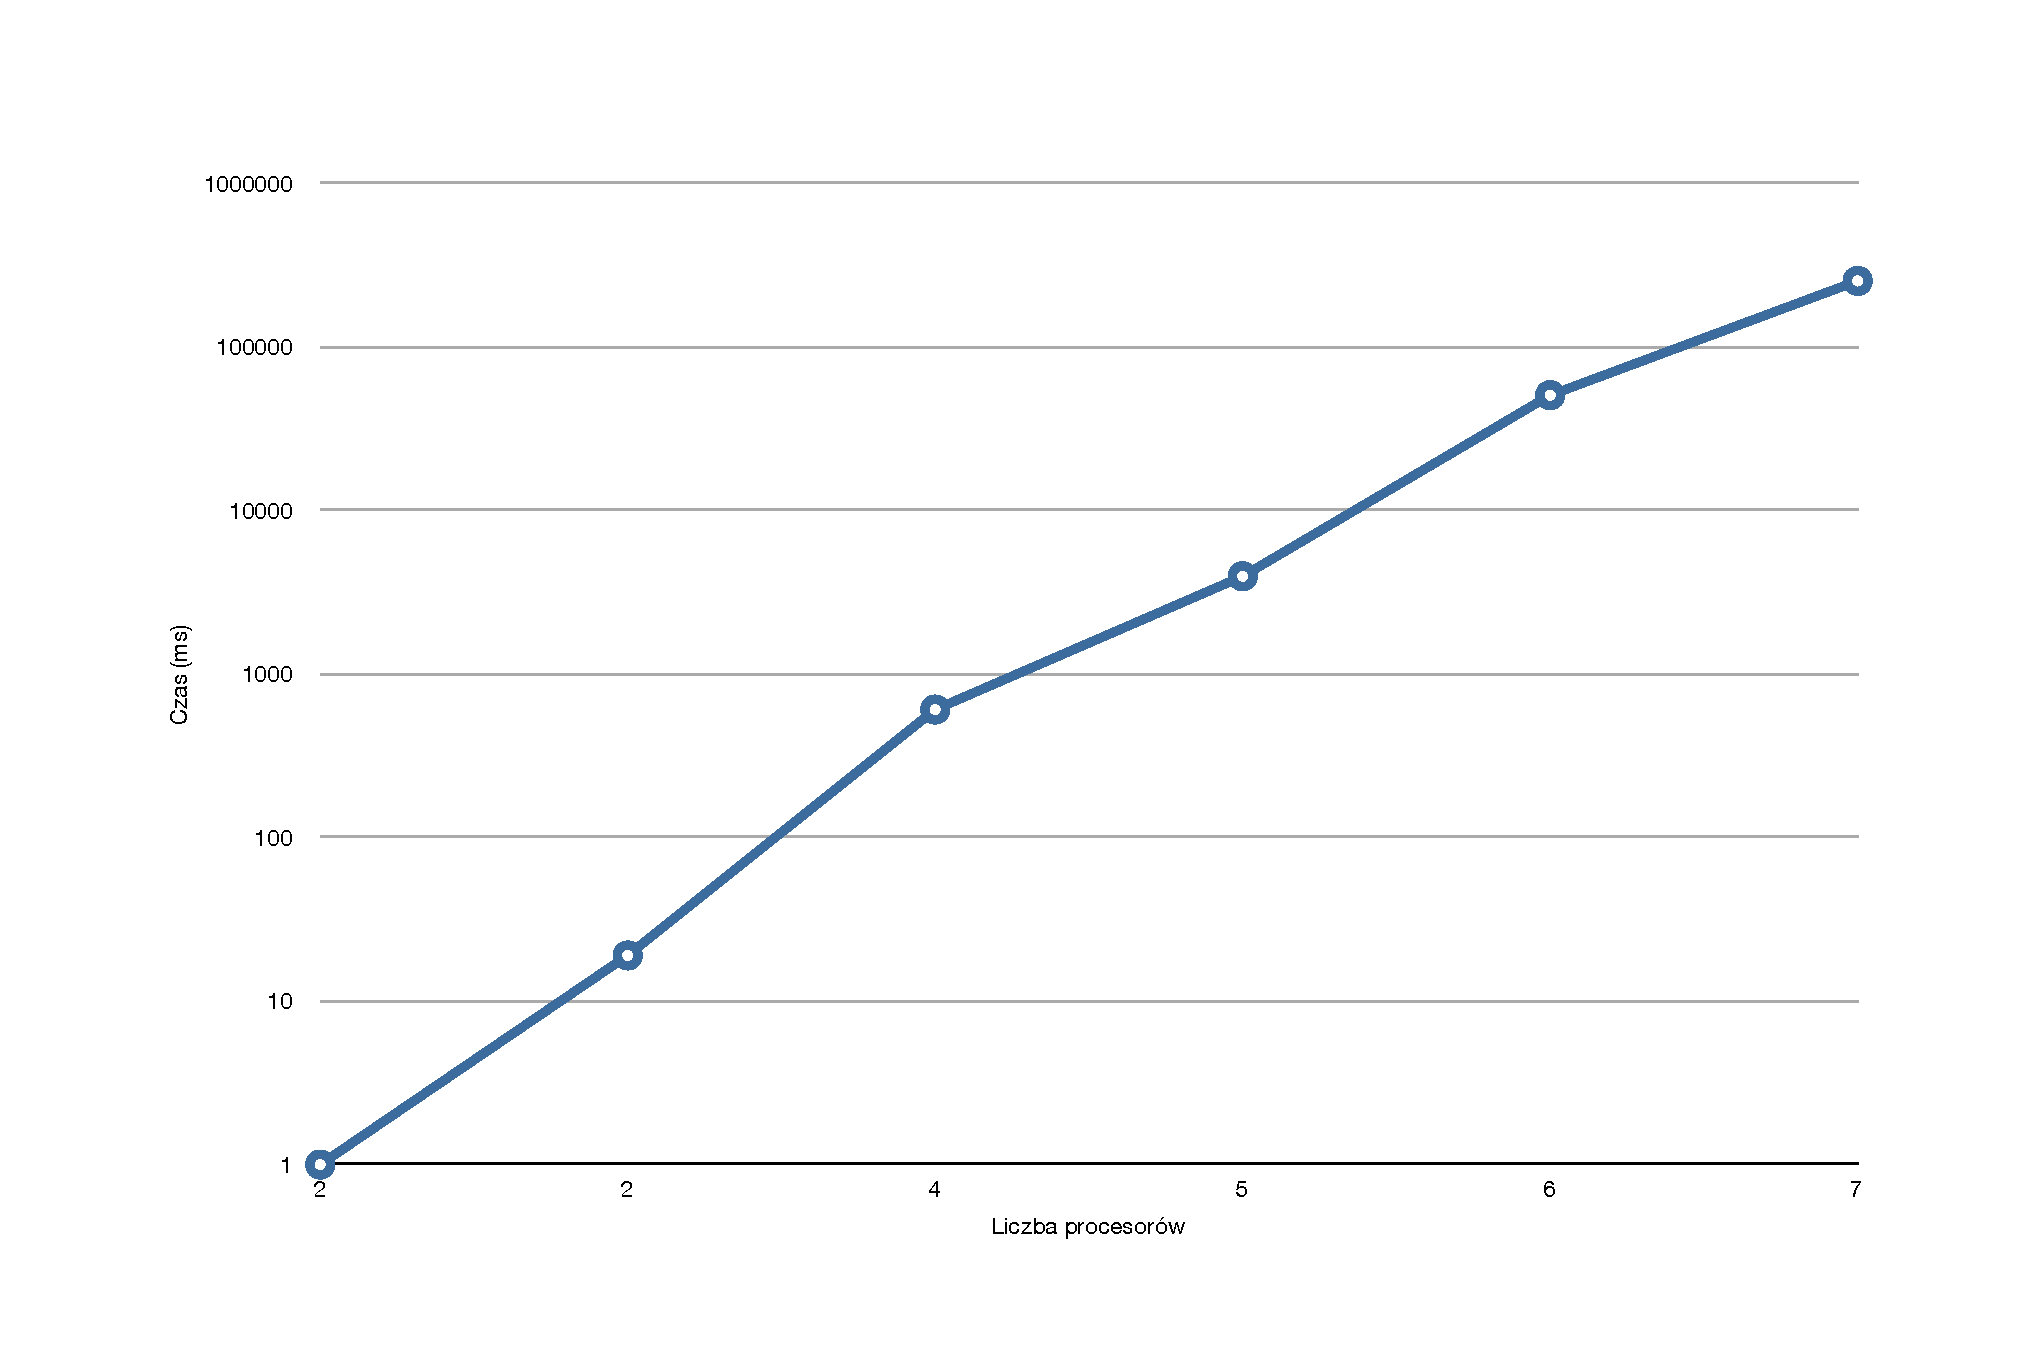
\includegraphics[width=\textwidth]{Fig2.pdf}
        \caption{}
	\label{fig2}
      \end{center}
    \end{figure}

    \begin{center}
    \begin{tabular}{ |c|c| } \hline
      p & T \\ \hline
      2 & 1 \\ 
      3 & 19 \\
      4 & 606 \\
      5 & 3956 \\
      6 & 50652 \\
      7 & 253205 \\ \hline 
    \end{tabular}
     
    \end{center}
    
    Jak widać na przestawionych wykresach (Rysunek \ref{fig1}, Rysunek \ref{fig2}) wraz ze wzrostem ilości procesorów, następuje wykladniczy wzrost czasu operacji szeregowania. Wieksza ilość zadań powoduje wzrost czasu operacji o kolejne rzędy wielkości.  
    \newpage
    \subsection{Zmienna wartość $C_{max}$ i liczba zadań, stała ilość processorów}
    \subsubsection{$m=3$, $n \in \{1,...,20\}$, $range \in \{1,...,20\}$}
     \begin{figure}[htbp]
      \begin{center}
       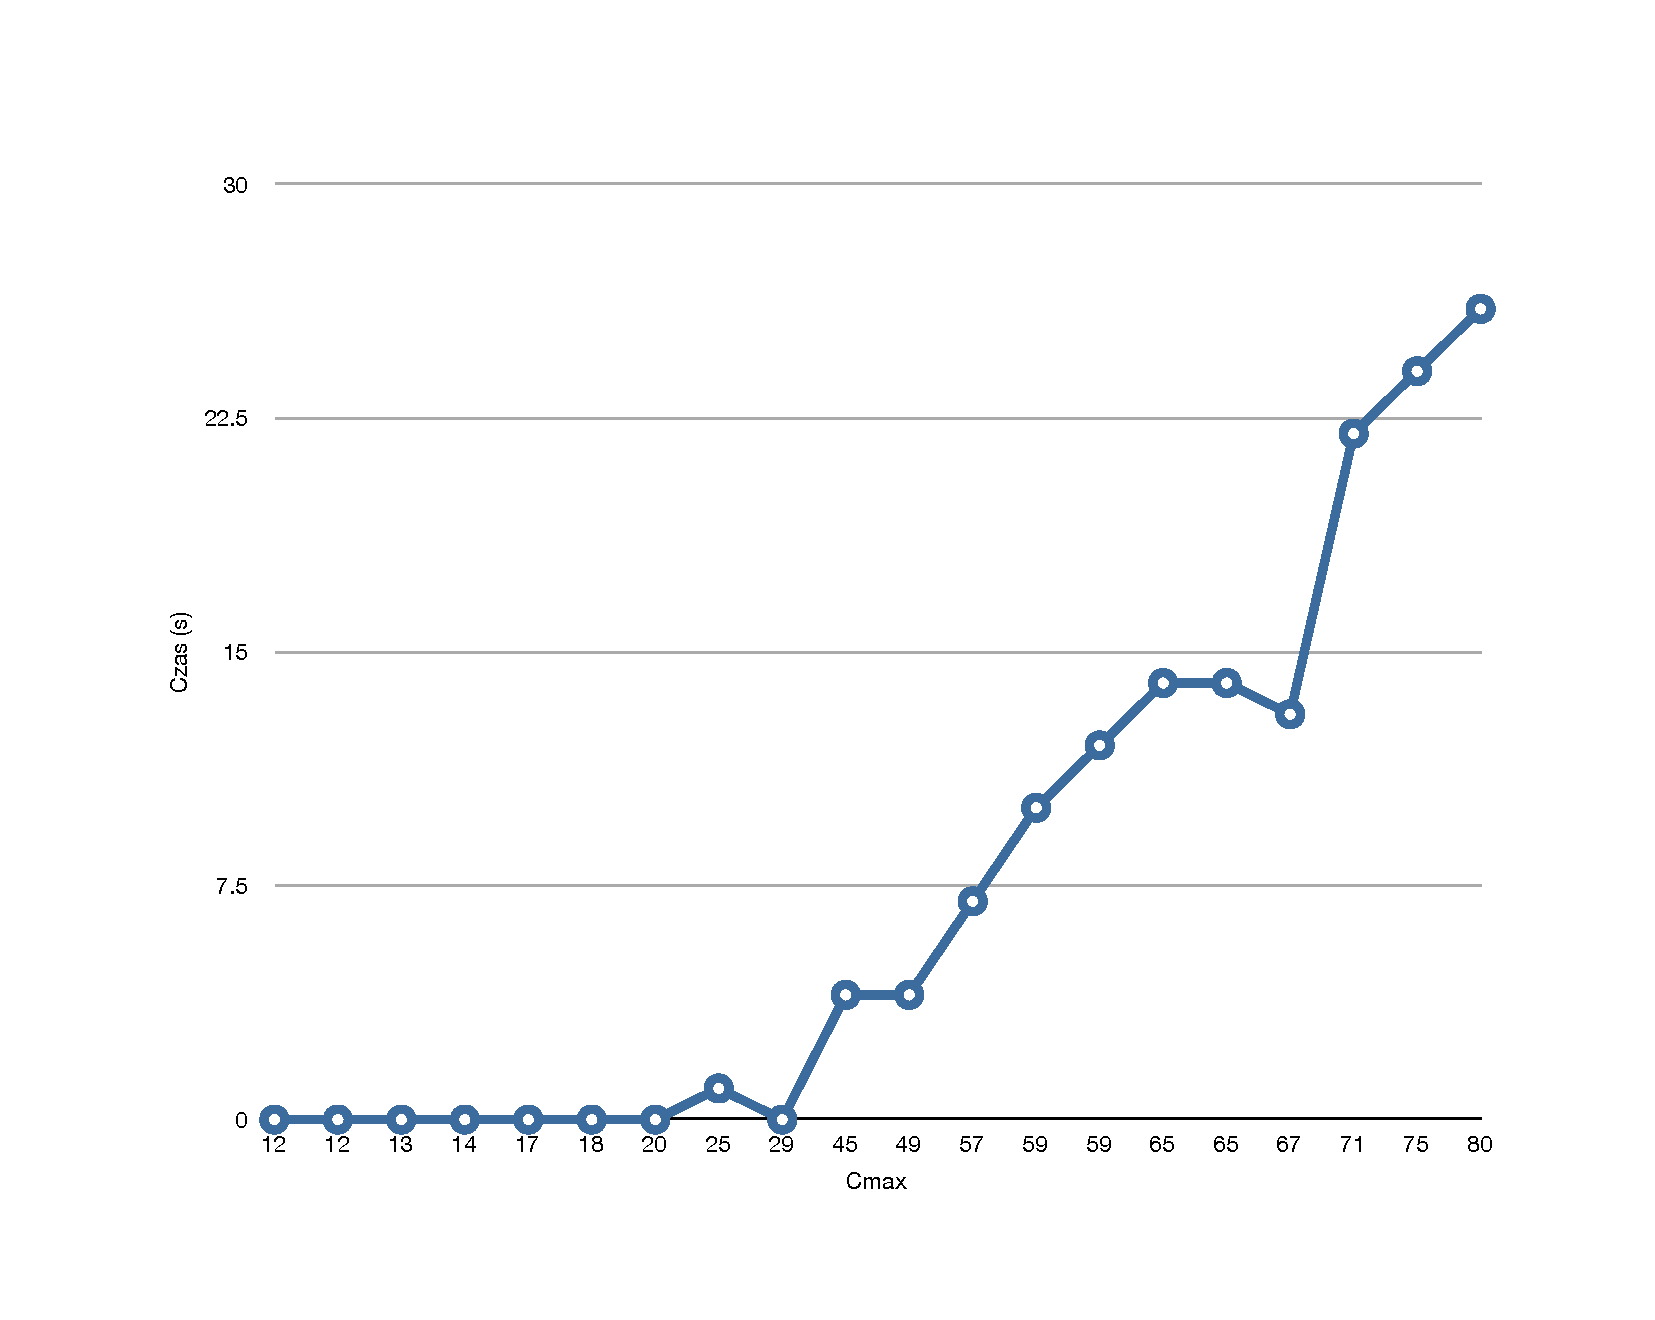
\includegraphics[width=\textwidth]{Fig3.pdf}
        \caption{}
	\label{fig3}
      \end{center}
    \end{figure} \newpage
    \subsubsection{$m=4$, $n \in \{1,...,20\}$, $range \in \{1,...,20\}$}
     \begin{figure}[htbp]
      \begin{center}
       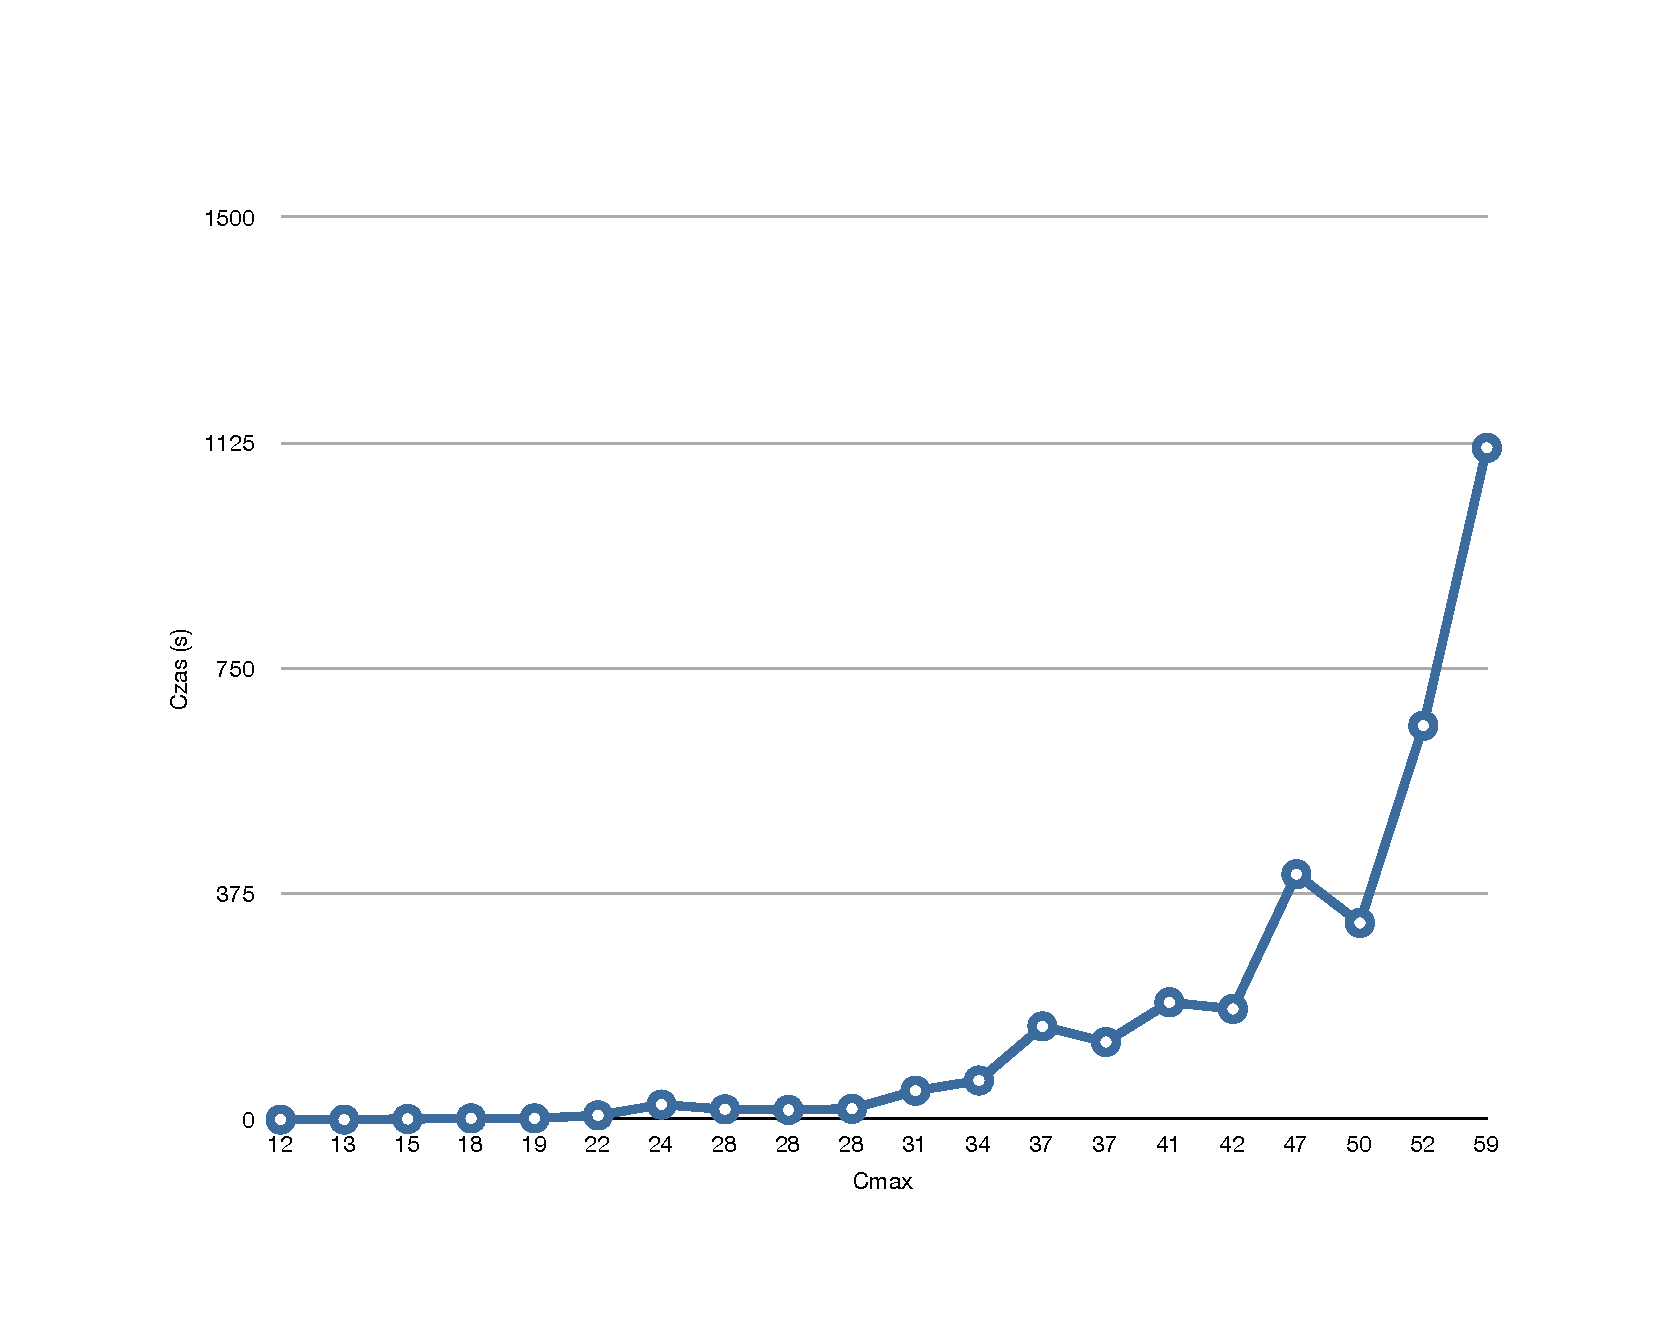
\includegraphics[width=\textwidth]{Fig4.pdf}
        \caption{}
	\label{fig4}
      \end{center}
    \end{figure} \newpage
    \subsubsection{$m=5$, $n \in \{1,...,20\}$, $range \in \{1,...,20\}$}
     \begin{figure}[htbp]
      \begin{center}
       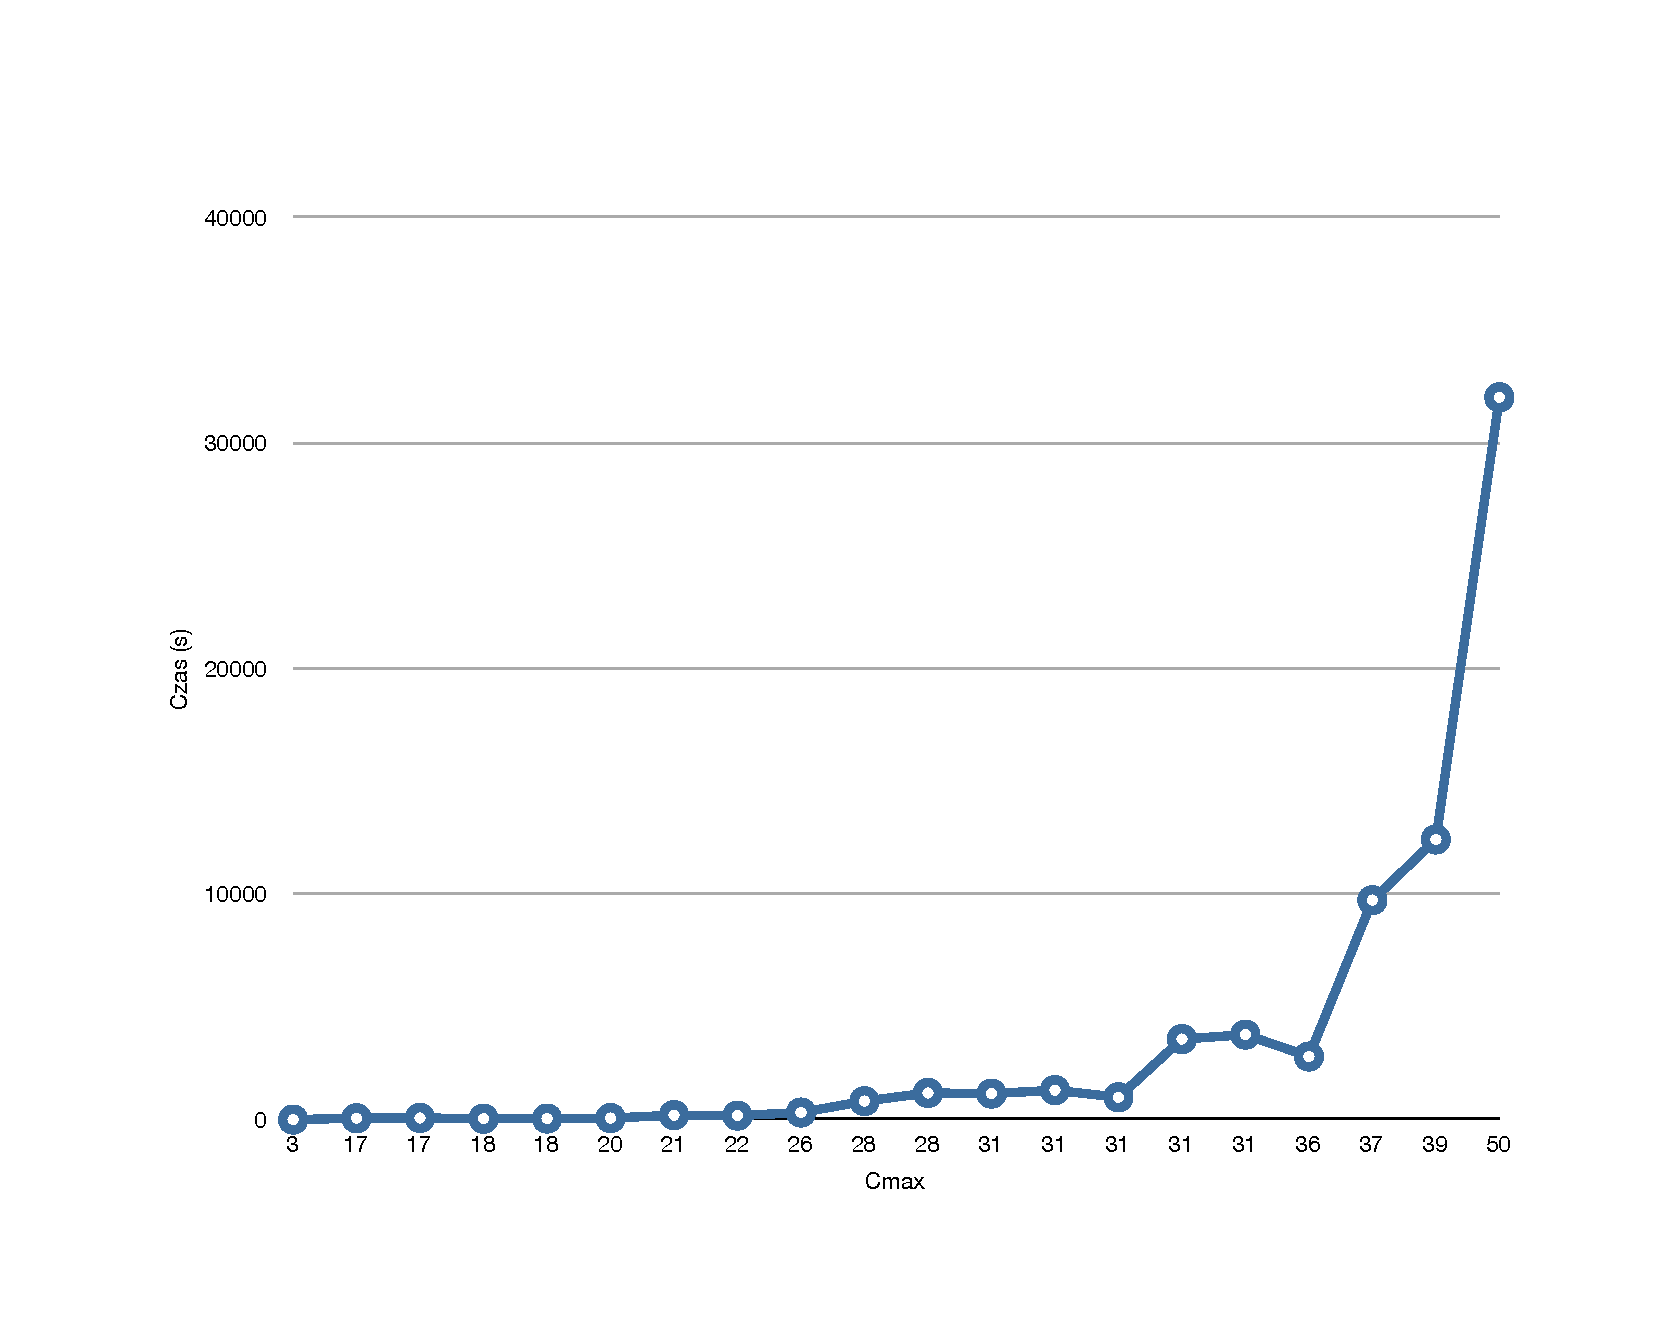
\includegraphics[width=\textwidth]{Fig5.pdf}
        \caption{}
	\label{fig5}
      \end{center}
    \end{figure}
    Powyższe wykresy (Rysunek 3, Rysunek 4, Rysunek 5) obrazują wpływ wartości $C_{max}$ na czas działania algorytmu. Dowodzi to wysokiej złożoności obliczeniowej algorytmu i wrażliwości na wielkość danych. 
\newpage
    \section{Wnioski}
\paragraph{}
     Zaimplementowany algorytm znajduje optymalne rozwiązanie zadanego problemu $NP-trudnego$, jednak wymaga relatywnie dużych zasobów (ilość dostępnej pamieci, szybkość procesora). Już dla małych wielkości algorytm wymagał większej ilości pamięci niż dostępna na testowym komputerze. Porównanie czasu wykonania z algorytmem naiwnym mija się z celem, ze względu na potrzebę uprzedniego obliczenia wartości $C_{max}$ za pomocą algorytmu $LPT$, aby ustalić parametry wejściowe algorytmu dokładnego. Wyniki maksymalnego czasu wykonywania wszytskich zadań po uszeregowaniu przy długościach zadań nie wiekszych niż $20$ (ograniczenia zasobów), nie rózniły się więcej niż o 3 jednostki. Nasuwa to wątpliwości co do potrzeby i opłacalności wykorzystania algorytmu dokładnego.    

\paragraph{}
Mimo iż program posiada interfejs graficzny, jego testy przeprowadzone zostały za pomocą aplikacji konsolowej, by zminimalizować narzut czasowy GUI na jakość i wartość otrzymanych wyników.

\end{document}


% \begin{figure}[htbp]
 %     \begin{center}
  %      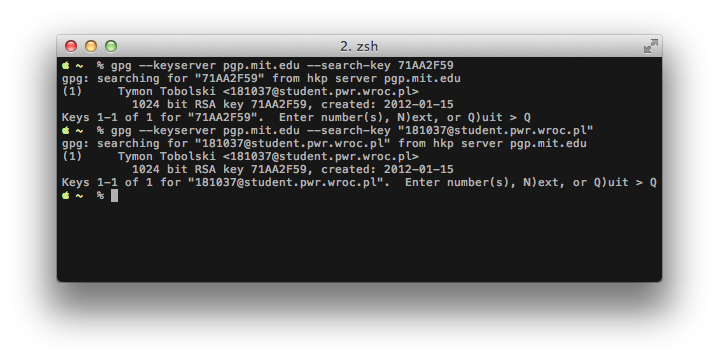
\includegraphics[scale=0.5]{screen/11.png}
   %     \caption{}
    %  \end{center}
    %\end{figure}